\section{Überblick über Open Innovation}\label{sec:grundlagen-open}

Das Modell der \textit{Open Innovation} ist -- schon rein namentlich -- der Gegensatz der \textit{Closed Innovation}.
Da der Fokus dieser Arbeit auf letzterem liegt,
wird im Folgenden der offene Ansatz lediglich oberflächlich behandelt.
\todo[inline]{... um später besser Vergleichen zu können?}

\begin{figure}[ht!]
    \centering
    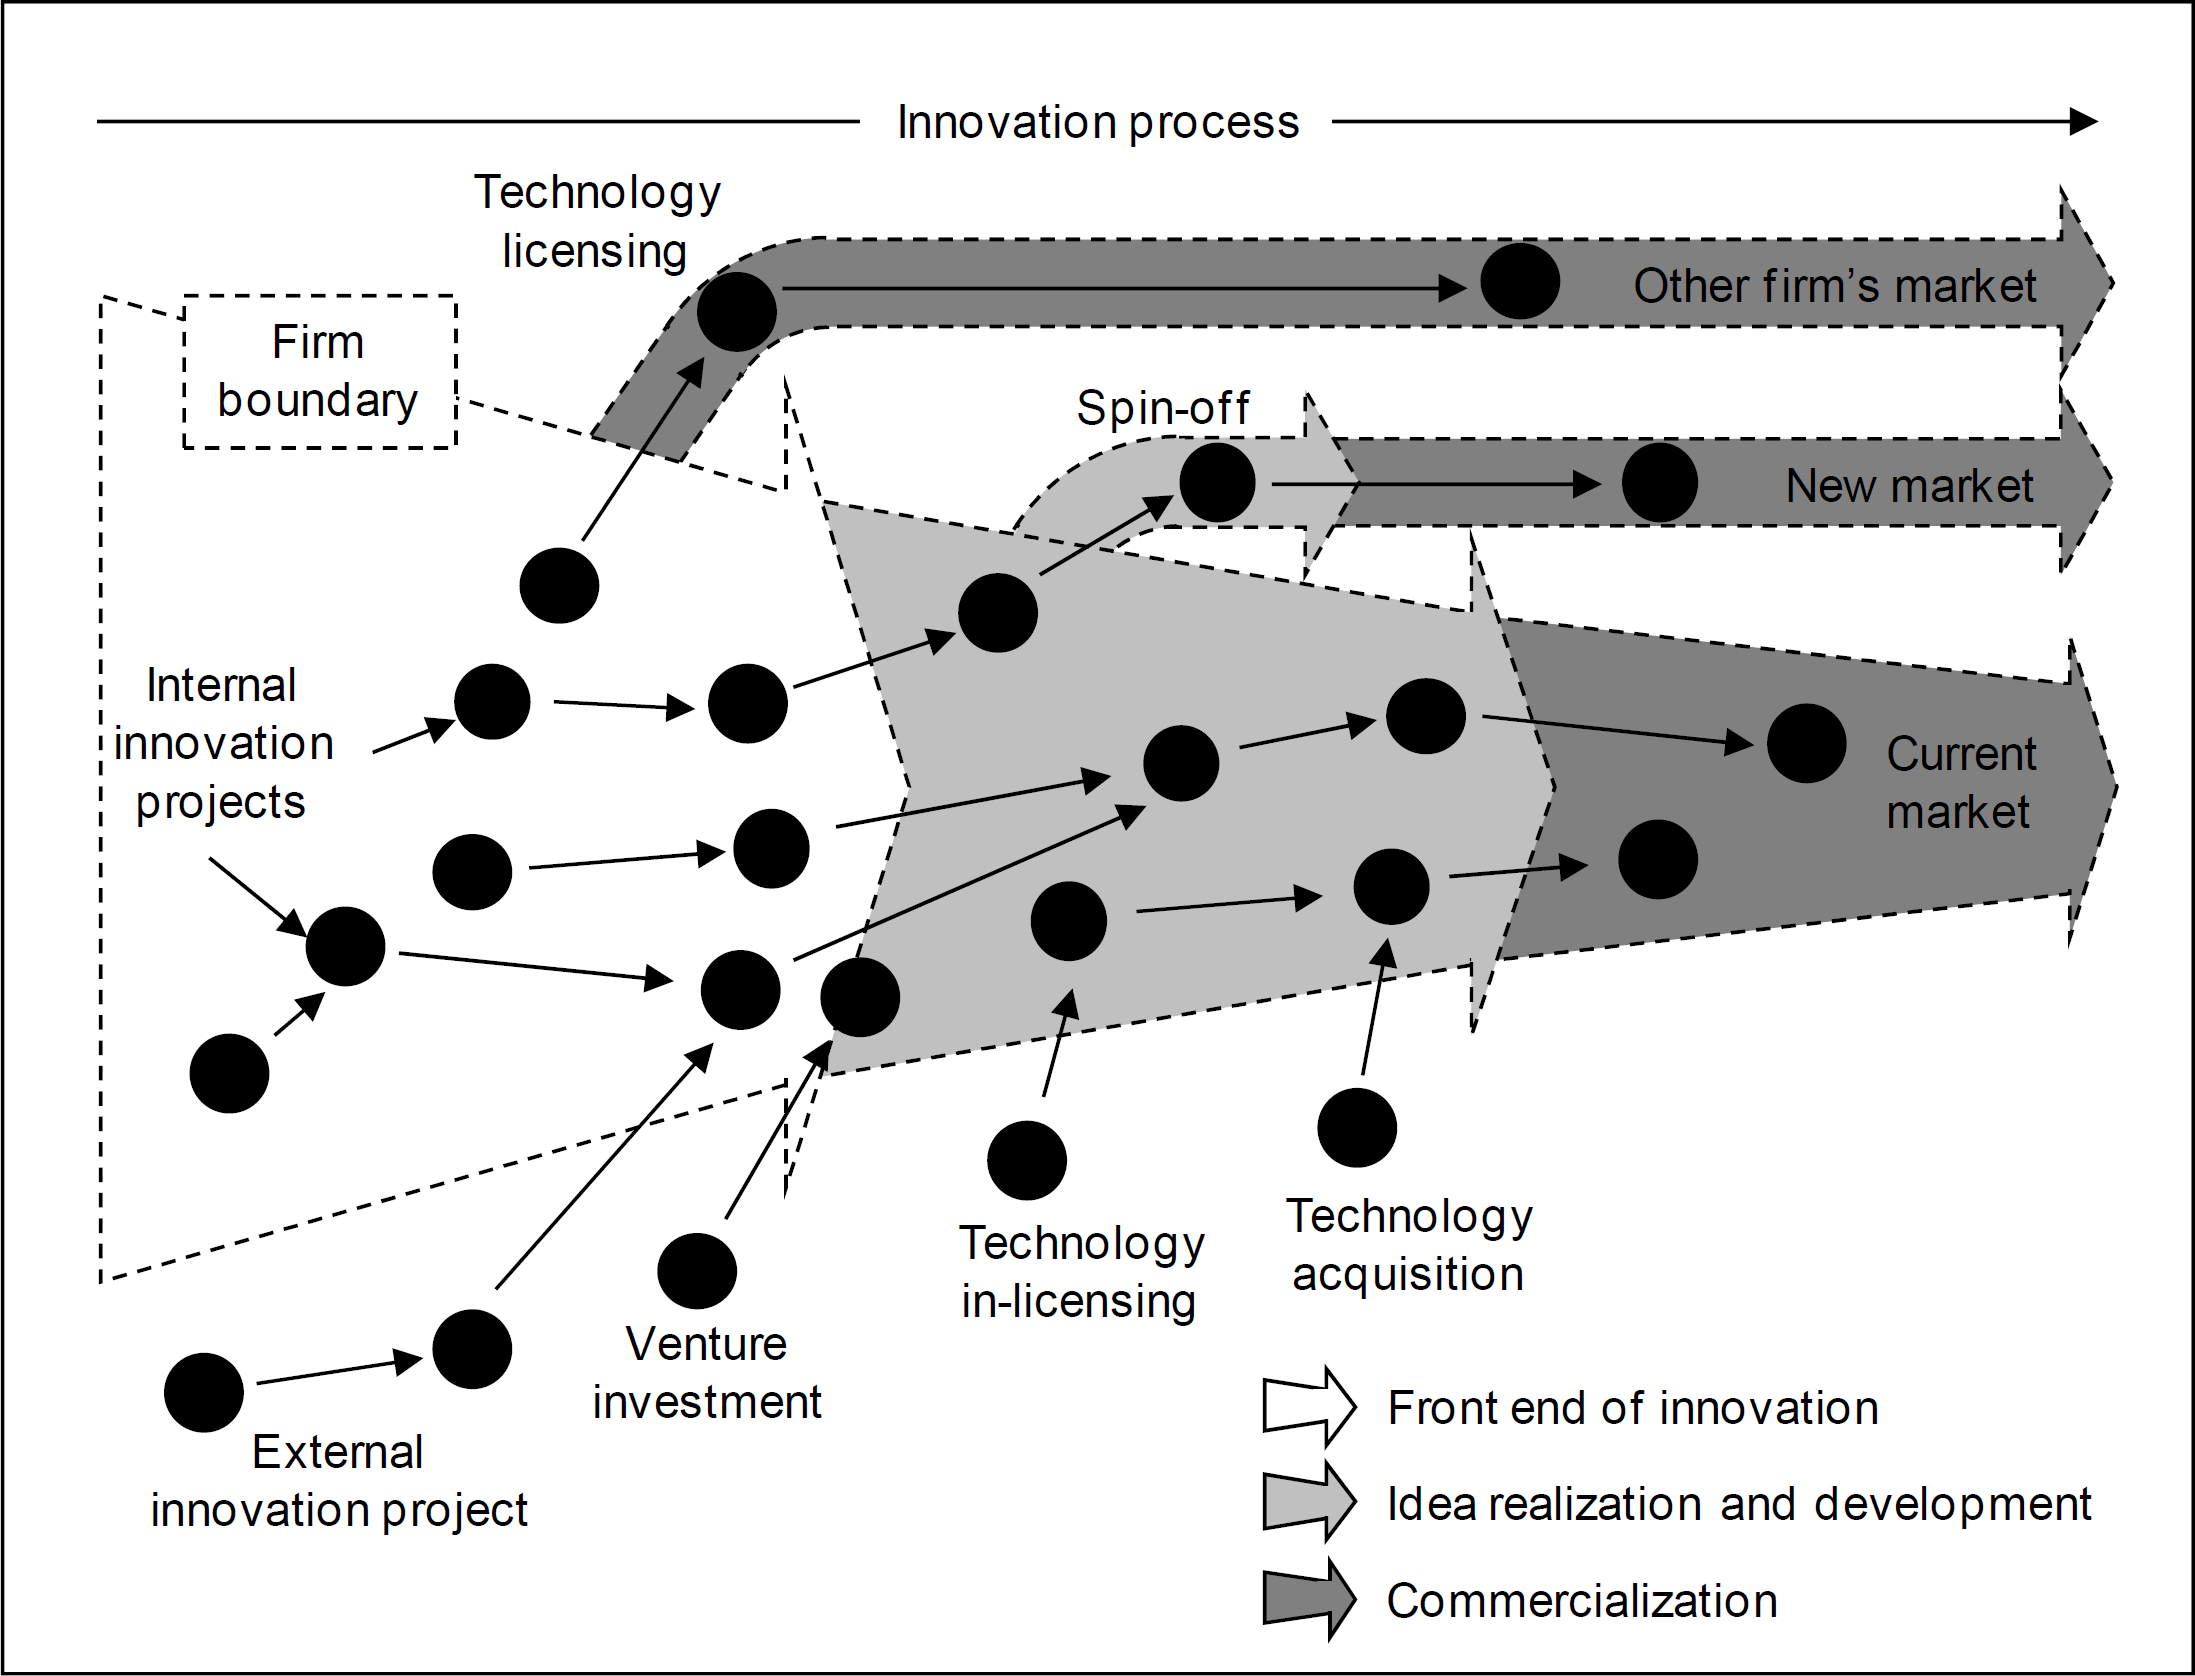
\includegraphics[width=1\textwidth]{OpenInnovation}
    \caption{Open Innovation Modell (aus \cite[23]{herzog2011})}
    \label{fig:openInnovation}
\end{figure}

Wie in \autoref{fig:openInnovation} zu sehen,
sind in der \textit{Open Innovation} die Grenzen eines Unternehmens \enquote{löchrig}.
Dies bedeutet, dass zusätzlich zu den intern entstandenen und entwickelten Innovationen
zusätzlich jederzeit Wissen von außen in den Innovationsprozess einfließt
und Projekte, welche innerhalb des Unternehmens nicht weiter verfolgt werden,
veröffentlicht werden oder genutzt werden um neue Märkte zu erschließen.

Details zum \textit{Closed Innovation}-Ansatz können in unter Anderem
in \cite[60\psqq]{chesbrough2003} und \cite[21\psqq]{herzog2011} nachgelesen werden.